% ------------------------------------------------------------------------------
% Este fichero es parte de la plantilla LaTeX para la realización de Proyectos
% Final de Grado, protegido bajo los términos de la licencia GFDL.
% Para más información, la licencia completa viene incluida en el
% fichero fdl-1.3.tex

% Copyright (C) 2012 SPI-FM. Universidad de Cádiz
% ------------------------------------------------------------------------------

% Las instrucciones de uso del \gls{framework} \gls{kf2} aplicado al \gls{strada} se detallan a continuación.

\section{\IfLanguageName{english}{Introduction}{Introducción}}
En el presente capitulo se desarrollará el manual de usuario, el cual permite obtener la información necesaria para los usuarios finales para poder utilizar el portal \gls{strada} en la versión implementada usando el \gls{framework} \gls{kf2}.\\

Esta aplicación web permite consultar las bases de datos de ``\transmov'' de los institutos del \glsfirst{dlr} \glsfirst{fw} y \glsfirst{vf} conjuntamente los documentos de ambos portales ofreciendo un sistema de búsqueda avanzada y optimizada sobre los \glspl{metadato} de los documentos de los institutos involucrados.\\

El portal ofrece una visualización del conocimiento interactiva de los \glspl{metadato}  que representa las relaciones espaciales, temporales y contextuales entre los documentos y fuentes de datos. Esta representación aporta nuevos conocimientos que facilitan las tareas de investigación.\\




Una vez concluida la instalación como se ha explicado en el capítulo \label{chapter:install}, la aplicación se encuentra preparada para ser usada siguiendo este manual.
\section{\IfLanguageName{english}{Features}{Características}}
% Recopilación de las principales funcionalidades del sistema.
Las principales funcionalidades de esta versión del \gls{strada} son las que se describen a continuación:
\begin{itemize}
	\item \textbf{Generación de grafo dinámico de exploración del conocimiento}
%	En usuario dispone en todo momento del grafo de exploración para la reprentación del conocmiento de la busqueda actual.
	\item \textbf{Complejidad personalizable del grafo de exploración}
%	El usuario puede seleccionar los grupos de elementos que serán representados en el grafo de exploración. De esta forma, se pueden generar grafos más complejos en base a las necesidades y \todo{sinónimo} gustos del usuario.
	\item \textbf{Búsqueda \gls{fulltext}.}
	\item \textbf{Búsqueda a través del grafo de exploración.}
	\item \textbf{Búsqueda a través del menú de opciones.}
    \item \textbf{Lista editable con los valores actuales de búsqueda.}
	% \item \textbf{Resaltado en los resultados de los valores buscados en \gls{fulltext}}
	\item \textbf{Pantalla de detalles por documento.}
    \item \textbf{\gls{url} con el estado de la aplicación compartible.}
    \item \textbf{Interacción visual de los elemento de la \gls{ui}.}
\end{itemize}


\section{\IfLanguageName{english}{Requirements}{Requisitos previos}}
% Requisitos hardware y software para el correcto uso del sistema.
Como se ha comentado anteriormente, es necesario la instalación previa de la aplicación. Los requisitos de ésta y los pasos a seguir se encuentran explicados en el capitulo anterior.\\

En lo que refiere al usuario del nuevo portal \gls{strada}, para poder acceder a él con una completa funcionalidad es necesario disponer de un navegador web actual con \gls{js} activo y que acepte \gls{html5}. Se recomienda el uso de \gls{chrome} o \gls{chromium} en sus últimas versiones aunque se pueden utilizar otros navegadores como \gls{ie} 9+, \gls{firefox} 32+ o \gls{safari} 5+.


\section{\IfLanguageName{english}{Using the System}{Uso del sistema}}
% Describir todos los aspectos necesarios para una utilización efectiva y eficiente del sistema por parte de los usuarios.
A continuación se describe cómo usar la aplicación y las posibilidades que ofrece. En la imagen \ref{image:manualgeneral} se observa  el emplazamiento de los componentes principales del portal \gls{strada}; grafo de exploración, menú de navegación, \gls{fulltext}, lista de resultados y selección actual. Los estilos de estos componentes están configurados para \gls{strada} siguiendo un código de colores que facilita la relación visual entre ellos.\\

Desglosado por estos componentes, se describe las acciones posibles a realizar con cada uno de ellos y las interacciones con el resto de elementos.

\begin{figure}[h!]
  \centering
  	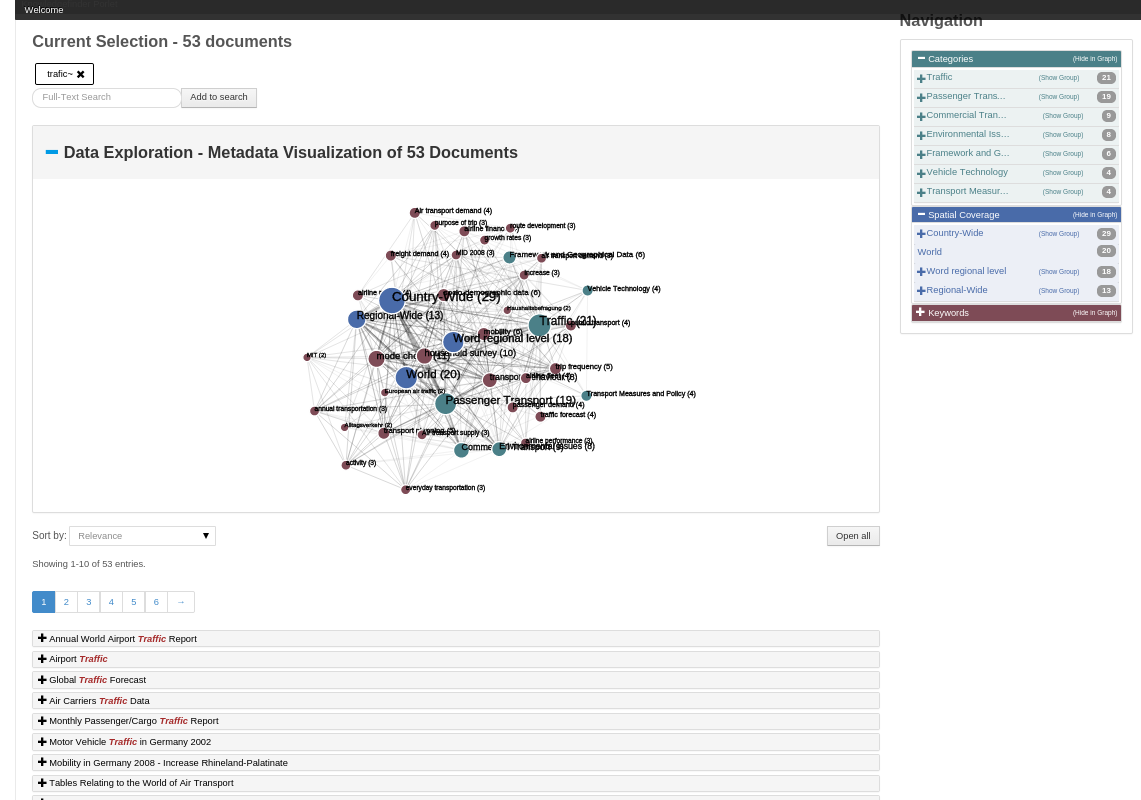
\includegraphics[width=1\textwidth]{general_ap.png}
  \caption{Pantalla principal del \gls{strada} usando \gls{kf2}}
  \label{image:manualgeneral}
\end{figure}

\subsection{Grafo de Exploración}
El grafo de exploración es el elemento principal de la visualización. Este está compuesto por nodos y por aristas que los unen. En la imagen \ref{image:manualgrafo} vemos un grafo de exploración con varios \glspl{metadato} interrelacionados.

\begin{figure}[h!]
  \centering
  	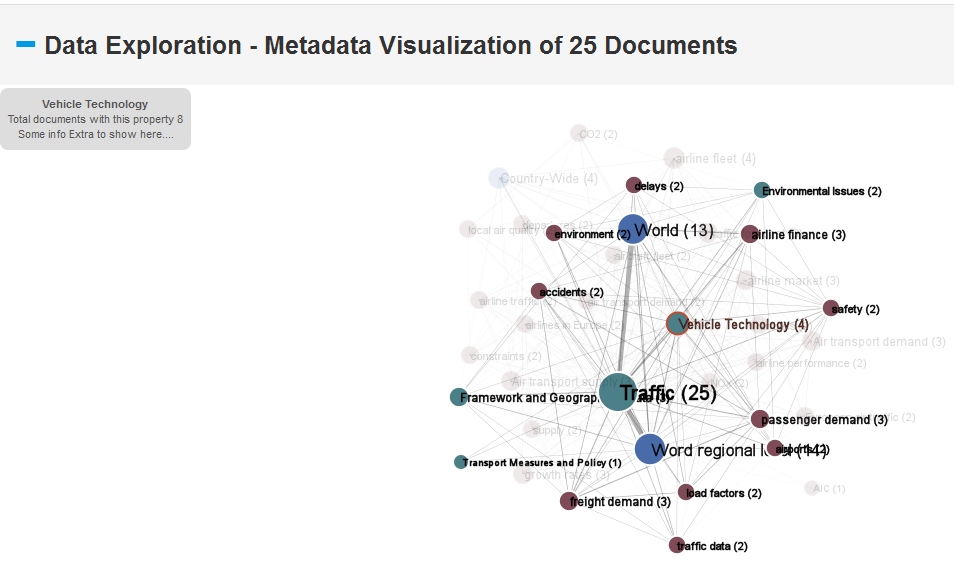
\includegraphics[width=0.8\textwidth]{graph1.png}
  \caption{Grafo de exploración de \gls{strada} usando \gls{kf2}}
  \label{image:manualgrafo}
\end{figure}

\subsubsection{Nodos}
Los nodos representan los filtros o \glspl{metadato} de los documentos y su tamaño varía dependiendo del número de documentos que los contentan para el actual conjunto de documentos.\\

Cuando se pulsa sobre uno de ellos, éste es usado para filtrar los documentos con este \gls{metadato}.\\

Por otra parte, mientras el usuario sitúa el cursor sobre uno de ellos (sin pulsar) todos los nodos del grafo no pertenecientes a su componente conexa (sin relación directa) se atenúan junto con sus relaciones y aparece un cuadro de texto con propiedades del \gls{metadato}. También se resaltan en la lista de resultados los títulos de los documentos con este filtro y en la menú de navegación el filtro.seleccionado. Por ejemplo, en la imagen \ref{image:manualgrafo} podemos ver con está resaltado en nodo \textit{Traffic} y los nodos con sus relaciones que están relacionados directamente con él. 

\subsubsection{Aristas}
Las aristas representan las relaciones entre \glspl{metadato} en función del número de documentos que contentan sus extremos. Mientras su grosor es directamente proporcional al a su valor, la longitud de la arista es inversamente proporcional.

Cuando se pulsa sobre una arista, su ambos \glspl{metadato} situados en sus extremos son aplicados para filtrar los documentos.\\

Si el usuario sitúa el cursor sobre una arista (sin pulsar) todos los nodos que no tienen ninguna relación con los extremos de la arista se atenúan y se muestra un mensaje con las propiedades de la arista. En la lista de resultados y en el menú se resaltan los elementos que contienen los \glspl{metadato} de los extremos.

\subsection{\fulltext}
%\todo{poner en otro lado?}
El formulario para la búsqueda \gls{fulltext} es el componente que proporciona versatilidad a la búsqueda (imagen \ref{image:manualfulltext}. El texto introducido es buscado entre los valores campos \textit{title}, \textit{description}, \textit{authors} y \textit{keywords}. A continuación se describen las distintas formas que hay para utilizar los valores para la búsqueda.

\begin{figure}[h!]
  \centering
  	
\includegraphics[width=0.5\textwidth]{search.png}
  \caption{Campo \gls{fulltext} de \gls{strada} usando \gls{kf2}}
  \label{image:manualfulltext}
\end{figure}
\subsubsection{Simple search}
Por defecto, se busca los documentos que contiene los alguno valores introducidos. Por ejemplo, si se introduce los valores del código \ref{code:search1} se obtendrán los documentos con \textit{germany} o \textit{2002}.

\begin{listing}[H]
\begin{minted}[linenos,
               numbersep=5pt,
               frame=single,
               framesep=2mm]{prolog}
	
germany 2002
\end{minted}
	\caption{Ejemplo - Simple search}
	\label{code:search1}
\end{listing}

\subsubsection{Matched phrase search}
Usando las comillas dobles se busca los documentos que contiene los exactamente la frase introducida. Por ejemplo, si se introduce los valores del código \ref{code:search2} se obtendrán los documentos que contiene exactamente \textit{germany 2002}.

\begin{listing}[H]
\begin{minted}[linenos,
               numbersep=5pt,
               frame=single,
               framesep=2mm]{prolog}
	
"germany 2002"
\end{minted}
	\caption{Ejemplo - Matched phrase search}
	\label{code:search2}
\end{listing}


\subsubsection{Disjunctive search}
Al igual que la búsqueda simple, con el operador OR (en mayúsculas) se busca los documentos que contiene los alguno valores introducidos. Por ejemplo, si se introduce los valores del código \ref{code:search3} se obtendrán los documentos con \textit{germany} o \textit{2002}.

\begin{listing}[H]
\begin{minted}[linenos,
               numbersep=5pt,
               frame=single,
               framesep=2mm]{prolog}
	
germany OR 2002
\end{minted}
	\caption{Ejemplo - Disjunctive search}
	\label{code:search3}
\end{listing}

\subsubsection{Conjunctive search}
Usando el operador AND (en mayúsculas) se busca los documentos que contienen los valores introducidos. Por ejemplo si se introduce la cadena del código \ref{code:search4} se obtendrán los documentos que contienen ambos valores; \textit{germany} y \textit{2002}.
\begin{listing}[H]
\begin{minted}[linenos,
               numbersep=5pt,
               frame=single,
               framesep=2mm]{prolog}
	
germany AND 2002
\end{minted}
	\caption{Ejemplo - Conjunctive search}
	\label{code:search4}
\end{listing}

\subsubsection{Exclusive search}
Con los operadores - y NOT (en mayúsculas) buscar documentos que no contienen ciertos valores. Por ejemplo si se introduce la cadena del código \ref{code:search5} o del código \ref{code:search5} se obtendrán los documentos que contienen \textit{germany} pero no \textit{2002}.
\begin{listing}[H]
\begin{minted}[linenos,
               numbersep=5pt,
               frame=single,
               framesep=2mm]{prolog}
	
germany NOT 2002
\end{minted}
	\caption{Ejemplo - Exclusive search}
	\label{code:search5}
\end{listing}

\subsubsection{Wirdcard searches}
Con el uso de elementos comodines ? (para un carácter) y * (para múltiples caracteres o ninguno) en la cadena de búsqueda se pueden realizar consultas más complejas. A continuación se muestran algunos ejemplos con comodines:

\begin{itemize}
	\item Para buscar documentos con valores entre 2000 y 2009 se podría usar la cadena búsqueda en el cuadro de código \ref{code:search6}.
\begin{listing}[H]
\begin{minted}[linenos,
               numbersep=5pt,
               frame=single,
               framesep=2mm]{prolog}
	
200?
\end{minted}
	\caption{Ejemplo 1 - Wirdcard search}
	\label{code:search6}
\end{listing}
	\item Para obtener los documentos con \textit{german} o \textit{germany} se pueden usar los comodines al final de la cadena de búsqueda (código \ref{code:search7}). 
    \begin{listing}[H]
\begin{minted}[linenos,
               numbersep=5pt,
               frame=single,
               framesep=2mm]{prolog}
	
german*
\end{minted}
	\caption{Ejemplo 2 - Wirdcard search}
	\label{code:search7}
\end{listing}

	\item Los comodines también se pueden combinar entre ellos en una misma cadena de búsqueda para precisar el termino a buscar. La búsqueda del código \ref{code:search8} encontraría \textit{germany} pero \textit{german}.
\begin{listing}[H]
\begin{minted}[linenos,
               numbersep=5pt,
               frame=single,
               framesep=2mm]{prolog}
	
ge*man?
\end{minted}
	\caption{Ejemplo 3 - Wirdcard search}
	\label{code:search8}
\end{listing}
\end{itemize}


\subsubsection{Fuzzy searches}
Las búsquedas \textit{Fuzzy} ayudan  a encontrar palabras que se deletreen de forma semejante. Para ello hay que añadir el carácter \~{} a la cadena de búsqueda. Por ejemplo, con los valores del cogido \ref{code:search9} se encontraran correctamente los términos con \textit{deutschland} aunque no esté bien escrito.

\begin{listing}[H]
\begin{minted}[linenos,
               numbersep=5pt,
               frame=single,
               framesep=2mm]{prolog}
	
deutshland~
\end{minted}
	\caption{Ejemplo - Fuzzy search}
	\label{code:search9}
\end{listing}

\subsubsection{Field searches}
Las búsquedas se puende concretar para los campos \textit{title} \textit{description} y \textit{keywords}. Concretando los campos afectados se centra la búsqueda sólo en él. en el código \ref{code:search10} se muestra un ejemplo de buscar la cadena \textit{germany} sólo en el título.
\begin{listing}[H]
\begin{minted}[linenos,
               numbersep=5pt,
               frame=single,
               framesep=2mm]{prolog}
	
title:germany~
\end{minted}
	\caption{Ejemplo - Field search}
	\label{code:search10}
\end{listing}

Todas las búsquedas anteriormente mostradas se pueden combinar y agrupar entre ellas. Como ejemplo se muestran los códigos \ref{code:search11} y \ref{code:search12}. En el primero se buscan los documentos cuyo título tengan algo parecido a \textit{deutshland} y su descripción no contenga la palabra \textit{germany}. El segundo ejemplo se busca documentos con la palabra clave \textit{transport} o \textit{traffic} y su título \textit{germany}.

\begin{listing}[H]
\begin{minted}[linenos,
               numbersep=5pt,
               frame=single,
               framesep=2mm]{prolog}
               
title:deutshland~ AND (NOT description:germany) 
 
\end{minted}
	\caption{Ejemplo búsqueda combinada 1}
	\label{code:search11}
\end{listing}

\begin{listing}[H]
\begin{minted}[linenos,
               numbersep=5pt,
               frame=single,
               framesep=2mm]{prolog}
	
(keywords:transport OR keywords:traffic) AND title:germany
\end{minted}
	\caption{Ejemplo búsqueda combinada 2}
	\label{code:search12}
\end{listing}

\subsection{Menú de Navegación}

En menú de navegación representa todos los filtros posibles a aplicar sobre el conjunto de datos. Estos filtros se encuentran organizados en dos niveles desplegables y con un \gls{scroll} para las listas de elementos más largas.\\

El número de documentos que poseen cada filtro se muestra junto a éste y los elementos siempre están ordenados por este número. En la imagen \ref{image:manualmenu} se observa los diferentes estados en que los filtros se pueden encontrar.

\begin{figure}[h!]
  \centering
  	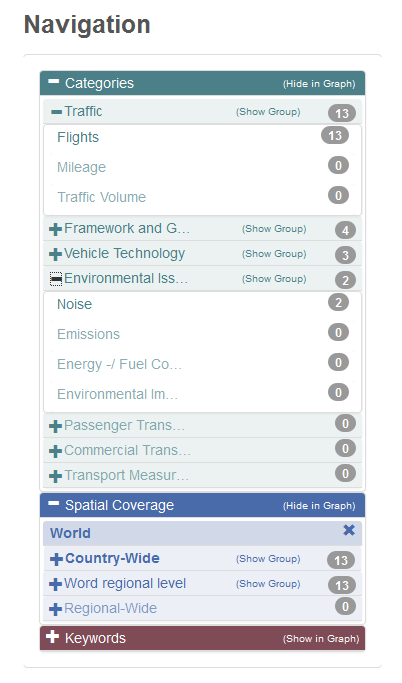
\includegraphics[width=0.5\textwidth]{menu.png}
  \caption{Menú de navegación de \gls{strada} usando \gls{kf2}}
  \label{image:manualmenu}
\end{figure}

\begin{itemize}
	\sitem{Filtro activo} Representa un \gls{metadato} el cual el usuario puede seleccionar pulsando sobre él. Se aplicará el filtro de búsqueda de este \gls{metadato} sobre el conjunto de documentos.
	\sitem{Filtro seleccionado} Filtro que está siendo usado entre los criterios de búsqueda. Pulsando sobre el icono $X$ de éste, el filtro se desactiva y éste vuelve a estar activo.
	\sitem{Filtro desactivado} Representa un filtro que no puede se usado para el conjunto de documentos actual ya que ningún documento lo tiene entre sus \glspl{metadato}.
\end{itemize}

En la imagen \ref{image:manualmenu} también se observan los elementos para configurar la complejidad del grafo de exploración (\textit{Hide in Graph} / \textit{Show in Graph} en las categorías principales y \textit{Show Group} / \textit{Hide Group}) en los grupos de filtros de segundo nivel. De esta forma, se pueden seleccionar los elementos que se desea ver representado en el grafo de exploración.

\begin{itemize}
	\sitem{\textit{Show in Graph}} Pulsando este botón se muestran, si procede, en el grafo de exploración los elementos del subnivel siguiente.
	\sitem{\textit{Hide in Graph}} Para ocultar en el grafo de exploración los elementos del primer subnivel pertenecientes a este conjunto de filtros, simplemente se debe pulsar este botón.
	\sitem{\textit{Show Group}} Se muestran en el grafo de exploración los subfiltros de este grupo.
	\sitem{\textit{Hide Group}} Se ocultan en el grafo de exploración todos los subfiltros de este grupo.
\end{itemize}

\subsubsection*{Interacción dinámica}
El usuario tiene la opción de usar este menú para interaccionar con el reto de componentes sin aplicar ningún filtro ni modificar los elementos mostrados en el grafo. Para ello, simplemente situándose sobre los elementos del menú sobre un filtro éste se marca con un círculo y los elementos que no pertenecen a su componente conexa se difuminan (ver imagen \ref{image:manualgrafo}. Junto al grafo aparece también un mensaje indicando propiedades del filtro implicado. A parte de ésto, en la lista de resultados se resaltan también los elementos que posen este filtro.

\subsection{Lista de Resultados}
La lista de resultados representa el conjunto de documentos ordenados que satisfacen los filtros de búsqueda que se aplican.\\

Esta lista está organizada a través de un sistema de \gls{paginacion} y puede ser reordenada. El usuario puede elegir entre algunas de las opciones del elemento \textit{dropdown} para personalizar el orden de la lista. Las opciones son:

\begin{itemize}
	\item{A-Z Title}: Alfabéticamente según el título del documento.
	\item{Z-A Title}: Alfabéticamente en orden inverso según el título del documento.
	\item{Relevante}: Por orden ascendente de puntuación en la búsqueda.
	\item{Actuality}: Ordenado por fecha de modificación ascendentemente.
\end{itemize}

La lista está diseñada con forma de acordeón. Se pueden expandir y contraer todos los elementos a través del botón \textit{Open all}/\textit{Close all} o pulsando sobre los títulos de los documentos. Cuando un elemento de la lista se encuentra expandido abierto se puede observar la descripción y el botón \textit{More Information} el cual muestra toda la información disponible del documento en una ventana emergente (imagen \ref{image:listaresults}).

\begin{figure}[h!]
  \centering
  	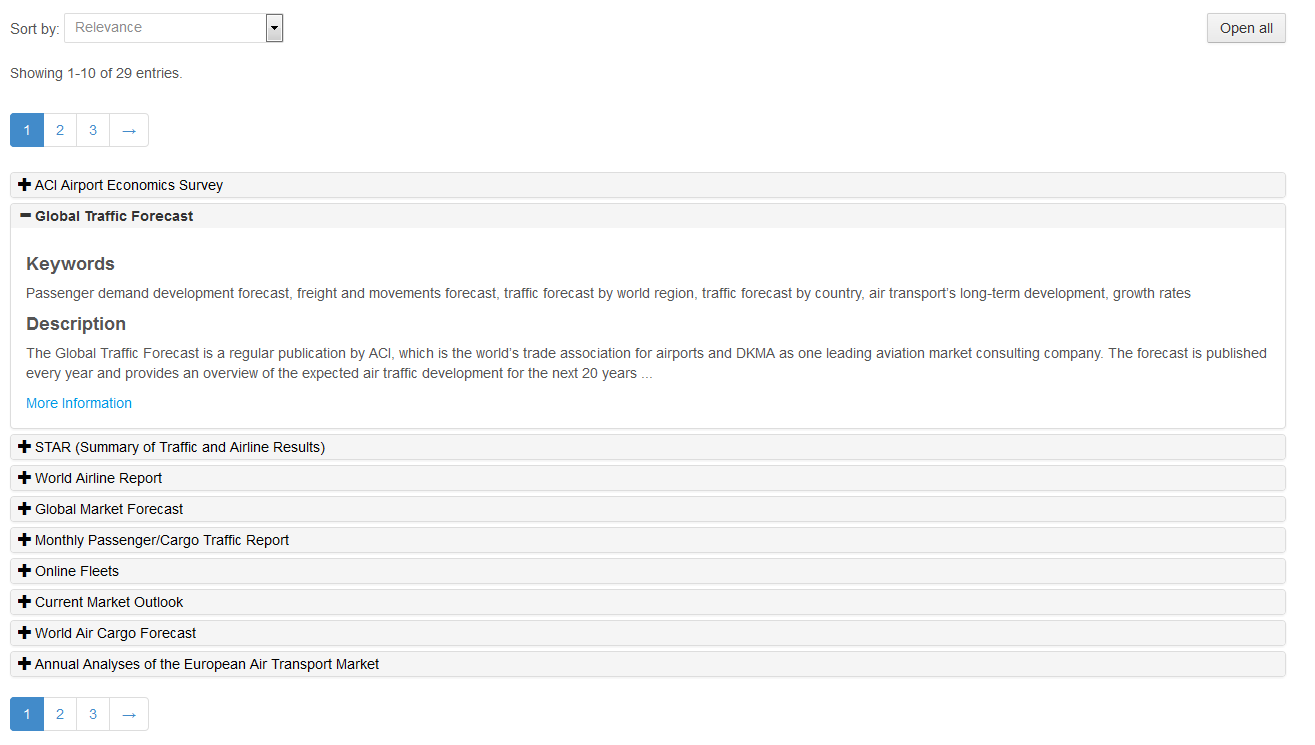
\includegraphics[width=1\textwidth]{results.png}
  \caption{Lista de Resultados}
  \label{image:listaresults}
\end{figure}

Tanto en la ventana emergente como los valores de la lista de resultados, si una búsqueda \gls{fulltext} se encuentra entre los valores de la consulta, las cadenas que coinciden con estas búsquedas son resaltadas. En las imágenes \ref{image:hightlist} y \ref{image:hightpop} se observa este comportamiento para la búsqueda de la cadena \textit{trafic\~{}} en la lista de resultados y en la ventana emergente de detalles respectivamente.

\begin{figure}[h!]
  \centering
  	
\includegraphics[width=1\textwidth]{highresult.png}
  \caption{Resaltado de \gls{fulltext} en la lista de resultados en \gls{strada} usando \gls{kf2}}
  \label{image:hightlist}
\end{figure}

\begin{figure}[h!]
  \centering
  	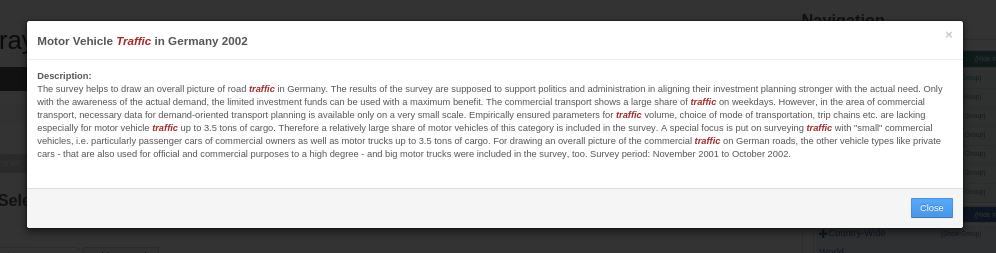
\includegraphics[width=0.7\textwidth]{hightpopp.png}
  \caption{Resaltado de \gls{fulltext} en la ventana emergente en \gls{strada} usando \gls{kf2}}
  \label{image:hightpop}
\end{figure}


\subsubsection*{Interacción dinámica}
Cuando el usuario se mueve sobre alguno de elementos de la lista de resultados, todos los nodos sin relación con este documento y sus relaciones son difuminados y en el menú de navegación son resaltados los \glspl{metadato} del documento afectado.

\subsection{Selección actual}
La selección actual (imagen \ref{image:manualselect}) es una lista de botones que representan los filtros que actualmente están activos y las cadenas de búsqueda introducidas a través del \gls{fulltext}.

\begin{figure}[h!]
  \centering
  	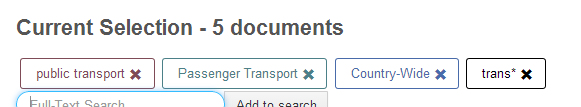
\includegraphics[width=0.7\textwidth]{current.png}
  \caption{Selección actual de \gls{strada} usando \gls{kf2}}
  \label{image:manualselect}
\end{figure}

Cuando se pulsa sobre alguno de ellos, el filtro se elimina de conjunto de filtros aplicados y este botón desaparece de la lista.


